\documentclass[11pt,letterpaper]{article}
\usepackage[utf8]{inputenc}
\usepackage{amsmath,amssymb,fullpage,graphicx}
\usepackage{subfigure}
\let\hat\widehat
\let\tilde\widetilde

\begin{document}
\subsection*{Q5-a}
\begin{verbatim}
bf_pvalue <- p.adjust(diet_pvalue$P.value, 'bonferroni')
data.frame(Variable=diet_pvalue$Dietary.Variable, Bonferroni.P = bf_pvalue)

            Variable Bonferroni.P
1     Total calories       0.0024
2          Olive oil       0.1920
3         Whole milk       0.9360
4         White meat       0.9840
5           Proteins       1.0000
6               Nuts       1.0000
7  Cereals and pasta       1.0000
8         White fish       1.0000
9             Butter       1.0000
10        Vegetables       1.0000
11         Skim milk       1.0000
12          Red meat       1.0000
13             Fruit       1.0000
14              Eggs       1.0000
15         Blue fish       1.0000
16     Carbohydrates       1.0000
17          Potatoes       1.0000
18             Bread       1.0000
19              Fats       1.0000
20            Sweets       1.0000
21    Dairy products       1.0000
22    Semi-skim milk       1.0000
23    Processed meat       1.0000
24        Total meat       1.0000
\end{verbatim}

\noindent This table shows adjusted p-values for each dietary variables by Bonferroni method. \\

\noindent Compare adjusted p-values to test size $\alpha = 0.05$. We can see each variables' adjusted p-value is larger than test size except for "Total calories". Therefore, we may conclude that only the p-value of total calories provided significant evidence for association between total calories and mammographic density. 

\newpage
\subsection*{Q5-b}
\begin{verbatim}
m <- nrow(diet_pvalue)
ordered_pvalue <- diet_pvalue[order(diet_pvalue$P.value),]
ben_pvalue <- rep(NA, m)
k_reject <- 0
for (ii in 1:m) { 
  adj_pvalue <- ordered_pvalue$P.value[ii] * m / ii
  ben_pvalue[ii] <- adj_pvalue
  if (adj_pvalue < 0.05) {
    k_reject <- ii
  }
}
> ordered_pvalue[1:k_reject,]
  Dietary.Variable P.value
1   Total calories   1e-04
\end{verbatim}
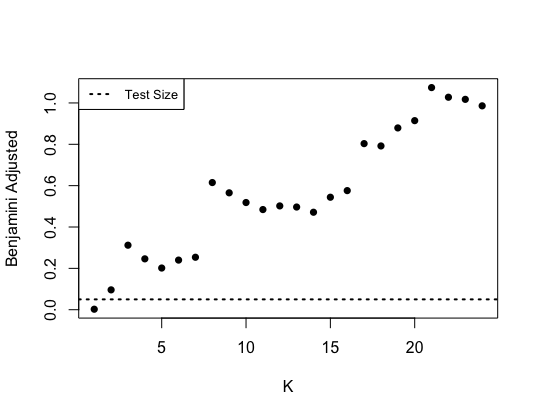
\includegraphics[scale=0.6]{q5-b.png}

\noindent The R code above calculated the larges $k$ such that $P_k \leq \frac{k}{m} FDR$, of which $k = 1$.\\

\noindent Both calculation and the plot show that given FDR $\alpha = 0.05$, the largest k such that $P_{k} \leq \frac{k}{m} \alpha$ is equal to 1 (in the plot, k=1 is the only point that has adjusted p-value less than FDR). So we can reject all $H_{0i}$ for $i = 1, ... k$, of which in this case $H_{0,1}$ is the only null hypothesis that can be rejected.\\

\noindent Therefore, we may conclude that observed data provides significant evidence that "total calories" is associated with mammographic density, but fail to provide significant evidence of associations between other dietary variables and mammographic density. \\

\noindent (R code in Appendix)

\end{document}